\documentclass[12pt,titlepage,a4paper]{article}

\usepackage[margin=0.5in]{geometry}
\usepackage{graphicx}
\usepackage{color}
\usepackage{amsmath}
\usepackage{amssymb}

\sloppy
\definecolor{lightgray}{gray}{0.5}
\setlength{\parindent}{0pt}

\title{Sharp(e) Selection Process \\
	\large Mean Variance Sharpe Ratio Analysis}
\author{
	Ariel Sosnovsky\\
	Victoria Tran\\
	Kosal Chhin\\
	Yossef Bisk}


\begin{document}

\maketitle
\section{Summary}
\subsection{What Does Our Program Do?}
\ \ \ Our program allows the user to find the most optimal portfolio for a given time period using the ‘mean variance optimization’ method. This program selects a portfolio of stocks from the global market that has minimum variance, as well as a maximized sharpe ratio.

\subsection{How Does The Program Do It?}
\ \ \ The program begins by partitioning the periods of a given time to smaller intervals. It then uses Yahoo Finance to download daily stock prices of over $30,000$ stocks traded on markets around the world. The stock data is then partitioned by industry and year with respect to indicated period, after which stocks which are missing more than $30\%$ of the data are removed from a given partition. Next the program enters the filtering stage. Where the existing set of stocks is divided into pairs of stocks that have the most negative correlation with each other, and then selects the top $25\%$ of pairs. Within that subset, the program selects the individual stocks with the top $25\%$ lowest variation. The portfolio now enters the selection stage. \\ \\
The selection stage is divided into two parts, which repeat as needed. The first part, addition part, we provide the program with a set of indices of the stocks within the market. If that set is empty then the stock with the lowest variance is added initially to the portfolio. Then the selection algorithm begins in which stocks are added to the portfolio only if they increase the Sharpe Ratio of the portfolio when the weights are optimized using the Mean variance optimization method, more than any other stock. Once a particular limit of stocks is reached, the algorithm ends. \\ \\
\ \ \  In the second part of the selection stage, the reduction part, the program will be provided with a set of indices of stocks. The program then will create every possible combination of portfolios with one less asset in it, than originally provided. Then the portfolio with the highest sharpe ratio is kept.  \\ \\ 
\ \ \ This stage will alternate between addition and reduction, until a convergence will occur. The resulting portfolio should be the minimum variance portfolio that offers the highest Sharpe ratio. 

\section{Introduction}
\subsection{Objectives and Motivation}
\ \ \ The goal of this paper is to test out how the classical mean variance portfolio (MVP) model with respect to the sharpe ratio performs, when applied to a large dataset. We start by developing a method of minimizing the variance of a portfolio with respect to the mean while searching for the maximum Sharpe ratio of a portfolio. Then, we test the method to a large data set and investigate the weaknesses of the model. The motivation for this is to investigate the model and its application and show how the results of the model stack up against criticism. We develop a selection purpose as a way to simulate real world application of the model. This sort of selection will theorectically reduce the transaction costs that one may incur while following a classical MVP approach. \\ 

\subsection{Background}
\subsubsection{Basics of Mean-Variance Portfolio Theory}
\ \ \  Mean variance optimization is a theory developed by Henry Markowitz in 1952, for portfolio optimization that has been standard for creating efficient asset allocation strategies for more than half a century. The theory aims at finding the optimal set of weights that achieves a desired expected return, $\mu_p$ from the portfolio with minimal risk $\sigma^2_p$. It does so, by defining a portfolio as a weighted average of market assets, $P = \sum_{j=1}^n w_j X_j$, and then uses methods of calculus to approximate the values of $w_j$ such that the variance function, $\sigma_p^2 = \sum_{j=1}^n\sum_{i=1}^nw_jw_iCov[X_i,X_j]$ is minimized with respect to a pre-set value $\mu_p$, where $\mu_p=\sum_{i=1}^nE[X_i]$.  It has also been widely criticized by many statisticians and economics for some of the assumptions that it makes on the mean and volatility of assets. As will be shown in this paper, the underlying issues that the assumptions of the model bring, become visible when the model is applied to a complete market. However, these problems become less severe as we reduce the intervals of time and increase the number of optimization instances.\\

\subsubsection{The Sharpe Ratio}
\ \ \  The Sharpe Ratio, developed in 1966 by William F. Sharpe, is a method of relating the portfolio return relatively to its risk. It is defined as: $Sharpe$ = $\frac{(\mu_p - r_f)}{\sqrt{\sigma_p^2}}$, where $r_f$ is the risk free interest rate given by the market or a government.  This is a measure for calculating risk-adjusted return, that is, the expected return earned in excess of the risk free rate per unit of standard deviation. In other words, for each risk we are taking, how much expected return are we getting out of it. But one of the problems with the Sharpe Ratio is that it treats all volatility the same, and this can result in penalizing upside volatility (potential of very high returns).\\

\section{Methodology}
\subsection{Mean-Variance Portfolio Optimization}
\subsubsection{Formulation of MVP}

To formulate the mean-variance problem, let us consider a simple bi-variate case for simplification, then we can generalize it to $n$ assets easily. To start, let the actual rate of return of asset $S_1$ and $S_2$ be $X_1$ and $X_2$ respectively. Then, the actual rate of return of our portfolio $P$ is:

$$
P = X_1w_1 + X_2w_2
$$
These are all random variables, so we can get the expected rate of returns and variances from historical data. And so we can get the expected rate of return of $P$: 

$$
E[P] = E[X_1w_1 + X_2w_2]
$$

By the linearity property of expectation, we get: 

$$
E[P] = w_1E[X_1] + w_2E[X_2]
$$
Let $E[P] = \mu_p$, $E[X_1] = \mu_1$, and $E[X_2]=\mu_2$ \\
So the expected rate of return of our portfolio is: 

$$
\mu_p = w_1 \mu_1 + w_2 \mu_2
$$
Which in matrix form is:
\begin{align*}
	\mu_p &= \mathbf{w}^T\pmb{\mu} \\
\end{align*}
Where,  $\mathbf{w}^T = [ w_1\ ,  w_2 ]$ and  $\pmb{\mu}^T = [ \mu_1\ , \mu_2 ]$. 
\\
Also, the expected risk (variance) is: 

$$
var(P) = var(X_1w_1 + X_2w_2)
$$

with sum of variance property: $$var(\sum_{i=1}^{n}{X_i}) = \sum_{i=1}^n\sum_{j=1}^{n}{Cov(X_i,X_j)}$$
we get: 
$$
var(P) = var(w_1X_1)+var(w_2X_2)+Cov(w_1X_1,w_2X_2)+Cov(w_2X_2,w_1X_1)
$$
we also know that: $Cov(X_1,X_2) = Cov(X_2,X_1)$, $var(w_iX_i)=w_i^2var(X_i)$, $var(X_1)=Cov(X_1,X_1)$ \\
Therefore: 
\begin{equation}
\begin{split}
var(P) &= var(w_1X_1)+var(w_2X_2)+2Cov(w_1X_1,w_2X_2) = \sum_{j=1}^2{{\sum_{i=1}^2w_jw_iCov(X_j,X_i)}}\\
\end{split}
\end{equation}
Let $var(P)=\sigma_p^2$, $var(X_i)=\sigma_{ii}^2$ and $Cov(X_i,X_j)=\sigma_{ij}^2$ \\ \\
In matrix form, (1) becomes: 
\begin{equation*}
\sigma_p^2 = \mathbf{w^T\Sigma w}
\end{equation*}
where $\mathbf{w} = \begin{pmatrix} w_1 \\ w_2 \end{pmatrix}$, and $\mathbf{\Sigma} = \begin{pmatrix}\sigma_{11}^2 & \sigma_{12}^2 \\ \sigma_{21}^2 & \sigma_{22}^2 \end{pmatrix}$ \\ \\ 
We are now ready to formulate the problem. We want the minimal risk with a certain expected rate of return $\mu_p$, while preserving our budget, therefore; we want to: 
\begin{equation}
\begin{aligned}
& \underset{w}{\text{minimize}}
& &\sigma_p^2 = \mathbf{w^T\Sigma w}\\
& \text{subject to}
& & \mu_p = \mathbf{w}^T\pmb{\mu} \\
&&& \mathbf{w}^T\mathbf{1}=1
\end{aligned}
\end{equation}
Like mentioned above that this can be easily generalize to $n$ assets, doing so we get: 

\begin{equation}
\begin{aligned}
& \underset{w}{\text{minimize}}
& &\sigma_p^2 = \mathbf{w^T\Sigma w}\\
& \text{subject to}
& & \mathbf{w^T}\pmb{\mu} = \mu_p \\
&&& \mathbf{w^T1}=1
\end{aligned}
\end{equation}
where $\mathbf{w} = \begin{pmatrix} w_1 \\ \vdots \\ w_n \end{pmatrix}$, 
$\pmb{\mu} = \begin{pmatrix} \mu_1 \\ \vdots \\ \mu_n \end{pmatrix}$, $\mathbf{1} = \begin{pmatrix}1 \\ \vdots \\ 1 \end{pmatrix}$, and $\mathbf{\Sigma} = \begin{pmatrix}\sigma_{11}^2 & \dots & \sigma_{1n}^2 \\ \vdots & \ddots & \vdots\\  \sigma_{n1}^2 & \dots & \sigma_{nn}^2 \end{pmatrix}$ is the covariance matrix.\\ \\ 
It turns out that (3) is a quadratic problem which can be solved using one of the methods from constraint optimization problem. Some of those methods are: Frank Wolfe's method, active set method, interior point convex method, Lagrange method etc. Since (3) is a minimization problem with only equality constraints, we will use Lagrange method to solve for a solution $\mathbf{w}$ which is the weight of our portfolio. 

\subsubsection{Lagrange Method to Solve (3)}

To solve the constrained minimization problem (3), we first create the Lagrangian function 
$$
L(\mathbf{w}, \lambda_1, \lambda_2) = \mathbf{w^T\Sigma w} + \lambda_1(\mathbf{w^T}\pmb{\mu} - \mu_p) + \lambda_2(\mathbf{w^T1} - 1)
$$
There are only two Lagrange multipliers $\lambda_1$ and $\lambda_2$ because (3) has only two constraints. Lagrange Method requires taking derivative of $L(\mathbf{w}, \lambda_1, \lambda_2)$ with respect to every single variables and set them equal to 0, doing so we have: 
\begin{equation}
\begin{split}
\frac{\partial L(\mathbf{w}, \lambda_1, \lambda_2)}{\partial \mathbf{w}} &= 2\mathbf{\Sigma w} + \lambda_1\pmb{\mu} + \lambda_2\mathbf{1} = 0 \\
\frac{\partial L(\mathbf{w}, \lambda_1, \lambda_2)}{\partial \lambda_1} &=  \mathbf{w^T}\pmb{\mu} - \mu_p = 0\\
\frac{\partial L(\mathbf{w}, \lambda_1, \lambda_2)}{\partial \lambda_2} &= \mathbf{w^T1} - 1 = 0\\
\end{split}
\end{equation}

The number of variables is always equal to the number of asset $n$ + 2 (2 for the additional Lagrange multipliers we introduced). Therefore, (4) consists of $n+2$ linear equations in $n+2$ unknowns ($\mathbf{w}, \lambda_1, \lambda_2$). We can represent the system of linear equations using matrix algebra as: 
\begin{equation*}
\begin{pmatrix} 2\mathbf{\Sigma} & \pmb{\mu} & \mathbf{1} \\ \mathbf{\mu^T} & 0 & 0 \\ 1^T & 0 & 0 \end{pmatrix} 
\begin{pmatrix}
\mathbf{w} \\ \lambda_1 \\ \lambda_2
\end{pmatrix}
 = 
\begin{pmatrix}
\mathbf{0} \\ \mu_p \\ 1
\end{pmatrix}
\end{equation*}

or 
$$
\mathbf{My_w} = \mathbf{b_p}
$$

where
\begin{equation*}
\mathbf{M} = \begin{pmatrix} 2\mathbf{\Sigma} & \pmb{\mu} & \mathbf{1} \\ \mathbf{\mu^T} & 0 & 0 \\ 1^T & 0 & 0 \end{pmatrix}, 
\mathbf{y_w}=\begin{pmatrix}
\mathbf{w} \\ \lambda_1 \\ \lambda_2
\end{pmatrix} \text{,and }
\mathbf{b_p} = \begin{pmatrix}
\mathbf{0} \\ \mu_p \\ 1
\end{pmatrix}.
\end{equation*}
The solution for $\mathbf{y_w}$ is: 
\begin{equation}
\mathbf{y_w} = \mathbf{M^{-1}b_p}
\end{equation}
In $\mathbf{y_w}$, the first $n$ elements are the portfolio weight $\mathbf{w}$ for minimum variance. \\ \\
This minimization problem is the basis of the Markowitz's asset allocation strategies. However, we would also like to look into the Sharpe ratio for this problem. \\

\subsection{Maximization of Sharpe Ratio}
Recall the definition of the Sharpe ratio: $Sharpe$ = $\frac{(\mu_p - X_f)}{\sqrt{\sigma_p^2}}$. Therefore, we can also look at the portfolio asset allocation problem as maximization of the Sharpe ratio: 
\begin{equation}
\begin{aligned}
& \underset{w}{\text{maximize}}
& & Sharpe = \frac{(\mu_p - X_f)}{\sqrt{\mathbf{w^T\Sigma w}}} \\
& \text{subject to}
& & \mathbf{w^T}\pmb{\mu} = \mu_p \\
&&& \mathbf{w^T1}=1
\end{aligned}
\end{equation}

To solve the maximization problem (6), we are using a \textbf{bisection method} in search for an optimal weight. See appendix for the breakdown of the bisection method.  

\subsection{Bisection Method}
briefly describe it here.

\subsection{The Selection Process}
put selection stuff here.

\subsection{Flow Chart of Implementation}
insert flow chart stuff. 

\section{Data}
For this project, we decided to use real life financial market data aggregated from the Yahoo Finance website. It provides a more interesting result and tests the accuracy of the algorithm. We begin by describing the conditions imposed on the data before collection, our data-mining algorithm, and lastly what methods were used to deal with missing data.
\subsection{Collection}
Below is a list of criteria and their justification chosen to fulfil the project requirements. 
\begin{enumerate}
\item Years 2008-2012
\begin{itemize}
\item the stock data has daily open and closing prices from Jan 2008 to Dec 2012
\item the time period was chosen to avoid any large financial movements in the market (ex. the 2008 financial crisis and the 2007-past bubble before)
\end{itemize}
\item Stock by Sector
\begin{itemize}
\item stocks were organized by the following sectors: Basic Materials, Conglomerates, Consumer Goods, Financial, Healthcare, Industrial Goods, Services, Technology, and Utilities
\item this was done since the MVP algorithm would create a portfolio from each sector and then create a portfolio from those portfolios
\end{itemize}
\end{enumerate}

\subsection{Mining Algorithm}
All the data was collected via a web-scraping algorithm programmed with R. The central idea of the program is to determine the URLs associated with each Yahoo Finance sector page with those the program can identify the stock symbol by inspecting the HTML content. See stocklist.R in the appendix.\\

After a list of stock symbols were created, the program then uses the function \textit{getYahooData} from TTR: (Technical Trading Rules) package in R to collect the historical prices. This process yields in total approximately 25,000 stocks. 
\subsection{Missing Data}
Unsurprisingly, there was missing data in some of the stock historical prices. This could be a due to a variety of factors: 
\begin{itemize}
\item Stock was split during some time in the year
\item Stock was newly created during some time in the year
\item Different exchanges operate in different counties, thus some stocks that only operate on specific exchanges might have a lag of information due to holidays
\end{itemize}

To resolve the problem, stocks who only had a minimum of 70\% of data were put in the selection pool. Here 70\% of the data is defined for the stock to have 180 entries since there are typically 256 working days in a given year.\\

For those stocks with empty entries, it was replaced with either the past day before closing price or the next day opening price depending on information available. This method is commonly used when repairing financial stock data.  


\section{Tests, Code and Results}

\begin{par}
For testing of our code we looked at how well our functions performed relative to the native matlab functions. For the selection algorithm we only used matlab as a benchmark, as there is no exisiting function that parrellels. Please note that all the tests found here can be found in the \texttt{Mean-Value-Opt/implementation/data\_matlabazer.m} file.
\end{par} \vspace{1em}

\subsection*{Data}

\begin{par}
We start by taking a random portion of data within our dataset, as follows:
\end{par}
\begin{verbatim}
	[Ret,CoRisk,stockNames,selData,data]=data_selector(folders,dates(1),sectors(6));
\end{verbatim}
\begin{par}
Note that \texttt{sectors(6)} is arbitrary sector name chosen from our sectors list, and \texttt{dates(1)}, is simply the data from \texttt{2008-2009}. This function will take the data from the folder, filter it, and then store it in the \texttt{selData} variable. Then it will compute the returns, and covariance and store them in the \texttt{Ret} and \texttt{CoRisk} variables respectively. The variable \texttt{data} is simply the unfiltered dataset.
\end{par} \vspace{1em}


\subsection*{Lagrange, Variance minimization method}

\begin{par}
\textbf{Overview}:
\end{par} \vspace{1em}
\begin{par}
Building on the mathematical theory we take the covariance matrix and the returns matrix and constructs the following matrices: Note that to ensure that the program does not run for too long, we control the number of assets we wish to test. If we wanted to test \textbf{all} of the assets we would set \texttt{n = length(Ret)}.
\end{par} \vspace{1em}
\begin{verbatim}n   = 100;
M   = Ret(1:n);
S   = 2.*CoRisk(1:n,1:n);
mp  = 0.05;\end{verbatim}
\begin{verbatim}A = [ S M' ones(n,1); M 0 0 ; ones(1,n) 0 0 ];
x = [ zeros(n,1); mp; 1 ];\end{verbatim}
\begin{par}
Hence, we can obtain the solution for our wieghts as follows: \texttt{Weights = A\ensuremath{\backslash}x};
\end{par} \vspace{1em}
\begin{par}
\textbf{Testing}:
\end{par} \vspace{1em}
\begin{par}
Next we will see how our function compares to the matlab base function \texttt{quadprog}. This will surve us as a benchmark for our function. The folllowing code will compare the matlab function to us.
\end{par} \vspace{1em}
\begin{verbatim}
mp  = 0.05;
n   = length(Ret);
S   = CoRisk(1:n,1:n);
M   = Ret(1:n);

% Matlab
tic
    w = quadprog(2.*S,[],[],[],[ M ; ones(1,n)],[mp;1],...
            [],[],[],...
            optimoptions('quadprog','Algorithm',...
            'interior-point-convex','Display','off'));
    fprintf('Matlab Time:  ');
toc

% Us
tic
    WW = [ 2*S M' ones(n,1); M 0 0 ; ones(1,n) 0 0 ]\[ zeros(n,1); mp; 1 ];
    fprintf('\nUs Time:  ');
toc

% Comparison
square_root_sum_of_error_squared = sqrt(sum((WW(1:end-2)-w).^2)./n)
\end{verbatim}

        \color{lightgray} \begin{verbatim}Matlab Time:  Elapsed time is 0.009409 seconds.

Us Time:  Elapsed time is 0.000961 seconds.

square_root_sum_of_error_squared =

   1.2973e-13

\end{verbatim} \color{black}
    \begin{par}
As you can see, our function outperformed the matlab function in terms of time. This is due to the fact that the matlab function runs several tests on the matrices before actually computing the weights.
\end{par} \vspace{1em}


\subsection*{Test Sharpe Optimization}

\begin{par}
The sharpe optimization procudure we wrote, makes use of the bisection method for finding the sharpe ratio. It is stored in the \texttt{optimizeSupreme} function. For more detail, please refer to the math-section of this paper. The matlab function we chose as the benchmark is the \texttt{estimateMaxSharpeRatio} which is a part of the \texttt{Portfolio Optimization and Asset Allocation} package in matab.
\end{par} \vspace{1em}
\begin{par}
We run our comparison code as follows:
\end{par} \vspace{1em}
\begin{verbatim}
clear n M S rfr WMp mLims
clc
n       = 10;
tP      = 1:n;
M       = Ret(tP);
S       = CoRisk(tP,tP);
rfr     = RFR(1);%list of risk-free rates (RFR(1) = 3.7%)
mLims   = 1E10;

% Matlab
tic
    p =  Portfolio('AssetMean',M,'AssetCovar',S,'RiskFreeRate',...
    rfr,'Budget',1,'LowerBound',-mLims,'UpperBound',mLims);
    WMp = estimateMaxSharpeRatio(p);
    Matlab_Sharpe = (M*WMp-rfr)/sqrt(WMp'*S*WMp)
    fprintf('Matlab Time:  ');
toc
% Us
tic
    [ sharpe, Wp, ~, ~ ] = optimizeSupreme( M, S, rfr );
    Our_Sharpe = (M*Wp-rfr)/sqrt(Wp'*S*Wp)
    fprintf('\nUs Time:  ');
toc
\end{verbatim}

        \color{lightgray} \begin{verbatim}
Matlab_Sharpe =

    0.0963

Matlab Time:  Elapsed time is 0.808331 seconds.

Our_Sharpe =

    0.0490


Us Time:  Elapsed time is 0.010628 seconds.
\end{verbatim} \color{black}
    \begin{par}
As you can see, our function outperformed the matlab function by a great deal. As a matter of fact, it performs significally better with higher values of \texttt{n}. However, our sharpe value seems to be at first glance much lower than matlab. This is beacuse we found a \textit{parrellel} portfolio to the one of matlab. To show what we mean by that, one may simply observe the ratio between the matlab weights and our weights:
\end{par} \vspace{1em}
\begin{verbatim}
disp(WMp./Wp);
\end{verbatim}

        \color{lightgray} \begin{verbatim}   1.0e+08 *

    5.3632
    5.1647
    5.0474
    5.1848
    5.8016
    5.2656
    4.9734
    5.1739
    5.3251
    4.9616

\end{verbatim} \color{black}
    \begin{par}
Or may look at the plot of the optimization period:
\end{par} \vspace{1em}
\begin{verbatim}
figure('Name','Our Optimization');
plot(Wp'*selData(:,1:n)')
title('Our Function');
xlabel('Time');
ylabel('Value of Portfolio');
figure('Name','Matlab Optimization');
plot(WMp'*selData(:,1:n)')
title('Matlab');
xlabel('Time');
ylabel('Value of Portfolio');
\end{verbatim}

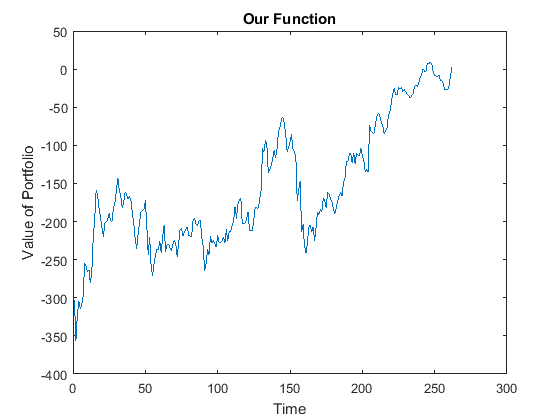
\includegraphics [width=3.5in]{testing_01.png}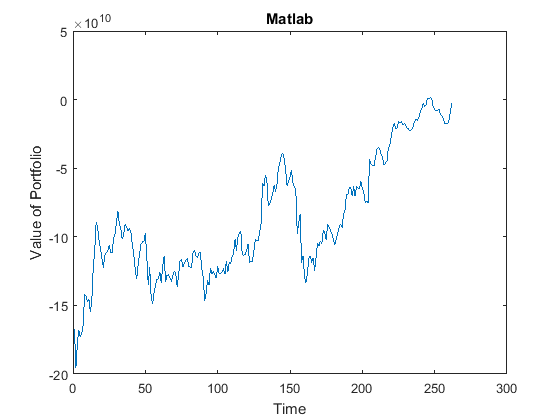
\includegraphics [width=3.5in]{testing_02.png}
\begin{par}
As you can see the only difference between our method and the matlab method is a multiplier. In this case the multiplier can be computed as approximately:
\end{par} \vspace{1em}
\begin{verbatim}
approximate_multiplier = mean(WMp./Wp)
WWW = approximate_multiplier.*Wp;
Our_Adjusted_Sharpe = (M*WWW-rfr)/sqrt(WWW'*S*WWW)
\end{verbatim}

        \color{lightgray} \begin{verbatim}
approximate_multiplier =

   5.2261e+08

Our_Adjusted_Sharpe =

    0.0929

\end{verbatim} \color{black}
    \begin{par}
Hence, our method compares well with matlab. As it provides us a good-enough estimate for the sharpe of the portfolio.
\end{par} \vspace{1em}
\section{Conclusion}
our method works well for short periods of time but not so much for long periods
Portfolio must be optimized frequently to avoid bad losses +++ obsviously mores stuff\\

\section{Discussion}
\subsection{Limitation of MVP in General}
\ \ \ One major limitation of the Mean Variance optimization technique is that it does not account for the constant changing of the parameters. This model treats the variances and covariances of stocks as constants when in essence they are variables. \\

\ \ \ Another issue with our method is that it does not account for transaction costs. Therefore, it is possible that the portfolio indicated as optimal based on a program is not really offer the optimal risk return ratio once transaction costs are factored into the equation.\\

\ \ \ Another related problem with MVP is that the solution can be unstable, in other words, small changes in inputs can result in huge changes in the portfolio weight. Because of this instability, a small change in the expected return can lead to entirely different portfolio weight. \\

\subsection{Future Study}
\ \ \ In the future, there are a couple of area methods we would like to study, that we can potentially use to revise and improve our project
One such way would be a Stop Loss method. In this method, our portfolio will be automatically re-optimized with the available data every time that the portfolio exceeds a specified level of loss. The reasoning behind this decision, is the relatively worsening performance of the portfolio as the duration since the last optimization increases. we theorize that this kind of more frequent 
optimization would make the portfolio more profitable.\\

\ \ \ We would also like to research the Black - Litterman model. The Black-Litterman model is a model used to estimate inputs for portfolio optimization. It mixes different types of estimates, some based on historical data, others based on equilibrium conditions to arrive at updated estimates. The Mixed Estimation Model was developed by Henri Theil in the early 1960's, but was applied to financial data by Fischer Black and Robert Litterman in the early 1990's.\\
\\
\ \ \ The beauty of this model is that one can blend a variety of views specified in different ways, absolute or relative, with a given prior estimate to generate a new and updated posterior estimate which includes all the views.  We feel that study this model would be a good next step at improving our project.\\

\ \ \ The MVP is known to be overly sensitive to estimation error in risk-return estimates and have poor out-of-sample performance characteristics. The Resampled Efficiency™ (RE) techniques presented in Michaud (1998) introduce Monte Carlo methods to properly represent investment information uncertainty in computing MVP portfolio optimality and in defining trading and monitoring rules.  we would like to study this technique in the future and perhaps integrate it into our program.\\

\section{References}

\section{Appendices}

\end{document}